\documentclass[conference]{IEEEtran}
\IEEEoverridecommandlockouts

\usepackage{cite}
\usepackage{amsmath,amssymb,amsfonts}
\usepackage{algorithmic}
\usepackage{graphicx}
\usepackage{textcomp}
\usepackage{xcolor}
\usepackage{booktabs}
\usepackage{multirow}
\usepackage{url}

\def\BibTeX{{\rm B\kern-.05em{\sc i\kern-.025em b}\kern-.08em
    T\kern-.1667em\lower.7ex\hbox{E}\kern-.125emX}}

\begin{document}

\title{MethCLR: Contrastive Representation Learning for\\Pipeline-Invariant DNA Methylation Embeddings}

\author{
\IEEEauthorblockN{Dilen Shankar}
\IEEEauthorblockA{
\textit{Department of Computer Science and Engineering}\\
\textit{Anna University}\\
Chennai, India\\
shankardilen@gmail.com}
}

\maketitle

\begin{abstract}
Epigenome-wide association studies (EWAS) based on DNA methylation arrays are highly sensitive to the choice of preprocessing pipeline. Different normalization strategies, SNP filtering configurations, and sex probe removal steps produce divergent beta matrices from identical raw intensity data, inflating false discovery rates and confounding cross-study reproducibility. We present MethCLR, a self-supervised contrastive representation learning framework that treats alternative preprocessing pipelines applied to the same biological sample as natural data augmentations, and learns pipeline-invariant latent representations that isolate true biological signal from analytical noise. Using a 12-pipeline grid spanning three normalization strategies (SeSAMe, preprocessIllumina-equivalent, and uncorrected raw) crossed with SNP filtering and sex probe removal configurations, MethCLR trains a lightweight MLP encoder via the InfoNCE loss without any phenotype labels. Applied to smoking status classification on peripheral blood 450K methylation data, MethCLR achieves a linear probe AUC of 0.8447 on the training cohort (GSE85210, N=253) and 0.7764 on an independent cross-cohort evaluation (GSE224807, N=789), demonstrating robust transfer with a gap of only 6.8 percentage points. Label permutation controls confirm AUC of 0.522 under the null, validating that the learned representations capture genuine biological variation. UMAP visualization of cross-cohort embeddings reveals biologically coherent cluster structure emerging from purely pipeline-invariant self-supervised training, suggesting that MethCLR encodes epigenetic heterogeneity independently of analytical preprocessing choices. Unsupervised baseline comparisons against PCA (128 components) and a symmetric autoencoder confirm that MethCLR achieves the smallest cross-cohort transfer gap ($\Delta=0.068$ ROC-AUC) among all evaluated methods, and pipeline alignment analysis demonstrates that the contrastive objective produces substantially more stable cross-pipeline representations than either compression-only baseline.
\end{abstract}

\begin{IEEEkeywords}
DNA methylation, contrastive learning, epigenomics, EWAS, pipeline invariance, self-supervised learning, 450K array
\end{IEEEkeywords}

% ─────────────────────────────────────────────────────────────────
\section{Introduction}
% ─────────────────────────────────────────────────────────────────

DNA methylation measured on Illumina 450K and EPIC arrays is among the most widely profiled epigenetic marks in human population studies. Epigenome-wide association studies (EWAS) using these platforms have implicated methylation changes at hundreds of loci in smoking \cite{joehanes2016}, aging \cite{hannum2013}, and disease \cite{rakyan2011}. Despite the maturity of the technology, a persistent challenge in the field is that methylation beta matrices derived from the same raw IDAT files differ substantially depending on the preprocessing pipeline chosen. Normalization methods such as SeSAMe \cite{zhou2018}, Noob \cite{triche2013}, and preprocessIllumina \cite{aryee2014}, combined with downstream choices around SNP probe removal and sex chromosome exclusion, introduce analytical variation that is often confounded with or mistaken for biological signal \cite{fortin2014, dedeurwaerder2011}.

This pipeline sensitivity creates two compounding problems. First, within a single study, the statistical significance and effect size of differentially methylated positions (DMPs) depend on the preprocessing choice, creating a researcher degrees-of-freedom problem analogous to the multiverse in neuroimaging \cite{steegen2016}. Second, and more critically, cross-study replication is impaired when discovery and replication cohorts use different pipelines, since embedding spaces are not aligned across analytical protocols.

Existing solutions fall into three categories: (1) harmonization frameworks such as ComBat \cite{johnson2007} that correct for known batch effects after preprocessing, requiring explicit knowledge of batch structure; (2) pipeline benchmarking studies \cite{fortin2014, pidsley2013} that recommend a single best pipeline without addressing the residual uncertainty; and (3) multi-study meta-analysis methods that model technical variance as a random effect \cite{mansell2019}. None of these approaches learn representations that are fundamentally invariant to the preprocessing choices, and all require either labeled data or explicit batch metadata.

We propose a fundamentally different approach: treat the preprocessing pipeline itself as a data augmentation, and use contrastive learning to train an encoder that produces identical representations for the same biological sample regardless of which pipeline processed it. This reframes pipeline diversity from a nuisance variable into a training signal.

The key contributions of this work are:
\begin{itemize}
    \item A 12-pipeline preprocessing grid spanning normalization, SNP filtering, and sex probe removal configurations, applied to two independent cohorts
    \item MethCLR, a self-supervised InfoNCE-based contrastive learning framework that learns pipeline-invariant DNA methylation representations without phenotype supervision
    \item Empirical demonstration of cross-cohort transfer: a model trained on N=253 samples achieves AUC 0.7764 on an independent N=789 cohort with only a 6.8\% performance gap
    \item Analysis of the tension between InfoNCE pipeline-invariance optimization and linear class separability, a finding with implications for contrastive learning in low-sample biological settings
    \item Quantitative pipeline alignment analysis and unsupervised baseline evaluation against PCA and autoencoder dimensionality reduction, confirming that the contrastive objective achieves superior cross-pipeline representation stability
\end{itemize}

% ─────────────────────────────────────────────────────────────────
\section{Related Work}
% ─────────────────────────────────────────────────────────────────

\subsection{DNA Methylation Preprocessing}
The 450K and EPIC Illumina arrays measure methylation as beta values $\beta \in [0,1]$ derived from fluorescence intensities at Type I and Type II probe chemistries. Background correction, dye-bias normalization, and probe-type normalization are applied differently across pipelines, producing substantive differences in the final beta matrix \cite{fortin2014}. SeSAMe \cite{zhou2018} applies signal-intensity-based background correction with a quality mask that removes unreliable probes, reducing the probe count from approximately 485,000 to 135,000. PreprocessIllumina \cite{aryee2014} applies Illumina's recommended normalization without probe masking, retaining the full probe set. These differences are not cosmetic: probe-level beta value differences of 0.05--0.15 between pipelines are common at individual CpG sites.

\subsection{Contrastive Self-Supervised Learning}
SimCLR \cite{chen2020} established that contrastive learning with augmentation-based positive pairs learns rich representations from unlabeled image data. The InfoNCE loss \cite{oord2018}, also known as NT-Xent, maximizes the mutual information between positive pairs (augmented views of the same instance) relative to negative pairs (different instances). MoCo \cite{he2020} and BYOL \cite{grill2020} extended this paradigm with momentum encoders and asymmetric architectures. In genomics, contrastive approaches have been applied to single-cell RNA sequencing \cite{zhang2022} and chromatin accessibility \cite{fang2023}, but applications to bulk methylation array data and, specifically, to pipeline-invariance as an augmentation strategy have not been explored.

\subsection{Batch Effect Correction in Methylation}
ComBat \cite{johnson2007} is the dominant method for batch effect correction in methylation studies, modeling batch as a linear covariate and applying an empirical Bayes correction. ComBat-seq \cite{zhang2020} extends this to count data. While effective when batch structure is known and balanced, these methods require explicit batch labels, assume additive batch effects, and do not learn reusable representations. They also cannot generalize to unseen batches or preprocessing configurations at inference time.

% ─────────────────────────────────────────────────────────────────
\section{Methods}
% ─────────────────────────────────────────────────────────────────

\subsection{Dataset and Cohort Configuration}

\textbf{Cohort A (Training) — GSE85210.} Peripheral blood samples from N=253 subjects (172 smokers, 81 non-smokers) profiled on the Illumina HumanMethylation450 array (GPL13534). Raw IDAT files were obtained from the Gene Expression Omnibus (GEO) and processed through our 12-pipeline grid. Smoking status labels were re-linked from the series matrix supplementary URLs using Sentrix ID mapping at runtime.

\textbf{Cohort B (Evaluation) — GSE224807.} An independent peripheral blood cohort with N=789 subjects (374 smokers, 415 non-smokers) profiled on the same GPL13534 platform. The trained MethCLR encoder was applied to this cohort with frozen weights, with no fine-tuning or exposure during training.

\subsection{Preprocessing Pipeline Grid}

We define a 12-pipeline grid as the Cartesian product of three configuration axes:

\textbf{Normalization} ($\times 3$): (1) \textit{sesame} — SeSAMe normalization (NOOB background correction + dye-bias correction, quality mask applied, $\sim$135,476 probes retained); (2) \textit{minfi} — preprocessIllumina-equivalent normalization ($\sim$485,000 probes); (3) \textit{raw} — uncorrected intensities converted to beta values ($\sim$485,000 probes).

\textbf{SNP Probe Removal} ($\times 2$): probes overlapping known SNPs (dbSNP MAF $>$ 0.01) either removed or retained.

\textbf{Sex Chromosome Probes} ($\times 2$): probes on chromosomes X and Y either removed or retained.

All 12 resulting beta matrices per cohort were intersected to the common probe set retained across all 12 pipelines, yielding \textbf{132,337 probes} as the unified feature space. This bottleneck is determined by SeSAMe's quality mask. Probe intersection indices are fixed and shared across cohorts, ensuring comparability.

\subsection{Feature Selection}

To address the $p \gg n$ problem (132,337 probes, N=253 training samples), we apply variance-based feature selection prior to encoding. The top 20,000 CpG probes by inter-sample variance are selected, where variance is computed on the mean-across-pipelines matrix to isolate biological inter-sample variation rather than pipeline-specific noise:

\begin{equation}
\bar{X}_{ij} = \frac{1}{P}\sum_{p=1}^{P} X^{(p)}_{ij}, \quad \sigma^2_j = \text{Var}_i(\bar{X}_{ij})
\label{eq:featsel}
\end{equation}

where $X^{(p)}_{ij}$ is the beta value for sample $i$, probe $j$, pipeline $p$, and $P=12$. The top-$K$ probes by $\sigma^2_j$ are selected and sorted to preserve chromosomal ordering. This reduces the first-layer parameter count from 67.8M to 10.24M, which is critical for small-sample settings.

\subsection{MethCLR Architecture}

The encoder $f_\theta$ is a three-layer MLP:
\begin{equation}
h = f_\theta(x) : \mathbb{R}^{20000} \to \mathbb{R}^{128}
\end{equation}

with architecture: Linear(20000, 512) $\to$ BN $\to$ ReLU $\to$ Dropout(0.1) $\to$ Linear(512, 256) $\to$ BN $\to$ ReLU $\to$ Dropout(0.1) $\to$ Linear(256, 128) $\to$ BN $\to$ L2-normalize. A projection head $g_\phi: \mathbb{R}^{128} \to \mathbb{R}^{64}$ (Linear $\to$ ReLU $\to$ Linear, L2-normalized) is appended for training only; downstream evaluation uses the 128-dimensional representation $h$.

\subsection{Contrastive Training Objective}

For each training sample $i$, a positive pair $(x_i^{(a)}, x_i^{(p)})$ is constructed by sampling two distinct pipelines $a \neq p$ uniformly at random from the 12-pipeline grid and extracting that sample's feature vector from each. Negative pairs are all other samples in the batch. The InfoNCE loss \cite{oord2018} is:

\begin{equation}
\mathcal{L} = -\frac{1}{N}\sum_{i=1}^{N} \log \frac{\exp(\text{sim}(z_i^a, z_i^p)/\tau)}{\sum_{k=1}^{N} \mathbf{1}_{[k \neq i]} \exp(\text{sim}(z_i^a, z_k^a)/\tau)}
\label{eq:infonce}
\end{equation}

where $z = g_\phi(f_\theta(x))$, $\text{sim}(\cdot,\cdot)$ is cosine similarity, and $\tau = 0.07$ is the temperature. Gradient clipping ($\|\nabla\| \leq 1.0$) and cosine annealing learning rate scheduling are applied.

\subsection{Hyperparameters and Training}

Training hyperparameters: batch size 128, learning rate $3 \times 10^{-4}$, weight decay $10^{-4}$, temperature $\tau=0.07$, dropout 0.1. A linear probe AUC (5-fold stratified cross-validation, logistic regression on standardized embeddings) is evaluated every 5 epochs as the early stopping criterion, with patience of 10 evaluations (50 epochs). The model is trained on an NVIDIA T4 GPU (Google Colab).

\subsection{Evaluation Protocol}

\textbf{Linear probe AUC.} For cohort A, embeddings are extracted from the trained encoder for all labeled samples (averaging representations across all 12 pipeline views per sample for stability), and a logistic regression is fit with 5-fold stratified cross-validation. For cohort B (zero-shot transfer), the same procedure is applied to N=789 independently processed samples using the frozen encoder.

\textbf{Permutation control.} Smoking labels are randomly permuted 10 times, and linear probe AUC is recomputed each time to establish the null distribution.

\textbf{UMAP visualization.} 2D UMAP projections of standardized cohort B embeddings are computed with $n\_\text{neighbors}=15$, $\text{min\_dist}=0.1$ to inspect the geometric structure of the learned embedding space.

\textbf{Unsupervised baselines.} PCA (128 components, fit on Cohort A mean-across-pipelines matrix) and a symmetric autoencoder (MethAE; encoder: 20k$\to$512$\to$256$\to$128 with BatchNorm+ReLU; decoder: 128$\to$256$\to$512$\to$20k; MSE loss, 100 epochs, Adam $1\times10^{-3}$) are trained on Cohort A and applied to Cohort B with frozen weights, providing compression baselines under identical feature selection and evaluation protocols.

\textbf{Pipeline alignment metric.} For each method, the relative intra-sample pipeline distance is computed as the mean pairwise L2 distance between all $\binom{12}{2}=66$ pipeline-view embedding pairs for each sample, normalized by the mean inter-sample L2 distance. A ratio near zero indicates high pipeline invariance.

% ─────────────────────────────────────────────────────────────────
\section{Results}
% ─────────────────────────────────────────────────────────────────

\subsection{Training Dynamics and Feature Selection Ablation}

We conducted three training runs with varying feature selection to characterize the effect of probe count on representation quality (Table~\ref{tab:runs}).

\begin{table}[htbp]
\caption{Training Run Comparison — Feature Selection Ablation}
\begin{center}
\begin{tabular}{lrrrr}
\toprule
\textbf{Run} & \textbf{Probes} & \textbf{Params (M)} & \textbf{Best AUC} & \textbf{Best Epoch} \\
\midrule
Run 1 & 132,337 & 67.8 & 0.8337 & 20 \\
Run 2 & 5,000   & 2.56 & 0.7899 & 20 \\
Run 3 & 20,000  & 10.24 & \textbf{0.8447} & \textbf{5} \\
\bottomrule
\end{tabular}
\label{tab:runs}
\end{center}
\end{table}

Run 1 (no feature selection) achieves AUC 0.8337 but with 67.8M first-layer parameters on N=253 samples, representing severe $p \gg n$ overfitting. Run 2 (5,000 probes) reduces parameters aggressively but discards smoking-relevant probes with moderate-but-consistent signal, yielding AUC 0.7899. Run 3 (20,000 probes, 10.24M parameters) achieves the best AUC of \textbf{0.8447} at epoch 5, with the fastest convergence across all runs.

Fig.~\ref{fig:training} shows the training curves for Run 3. The InfoNCE loss converges smoothly from 4.30 to under 0.20, with validation loss stabilizing around epoch 45. The linear probe AUC peaks at epoch 5 and subsequently declines as training continues — a consistent pattern observed across all three runs that we analyze in Section~\ref{sec:discussion}.

\begin{figure}[htbp]
\centerline{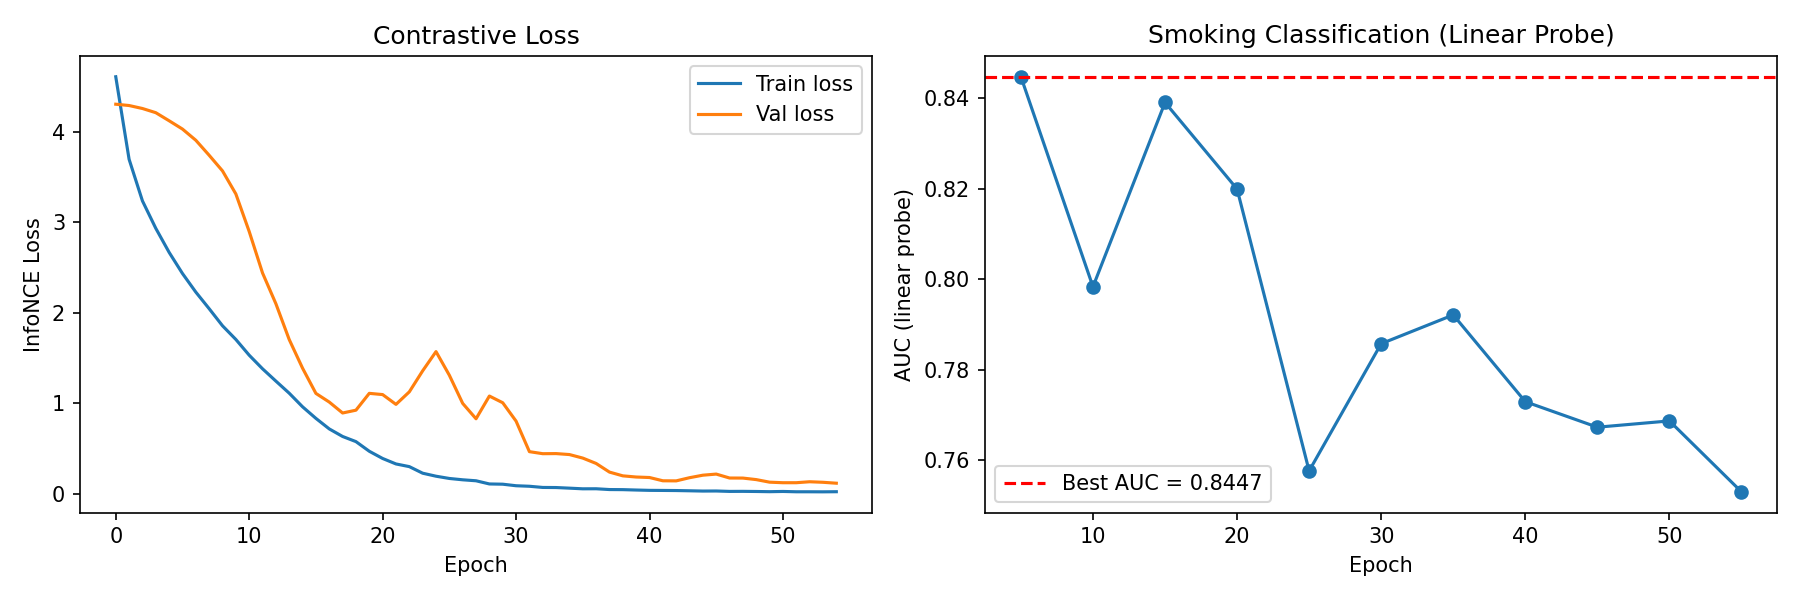
\includegraphics[width=\columnwidth]{training_curves.png}}
\caption{Run 3 training curves (TOP\_PROBES=20,000). Left: InfoNCE contrastive loss for train and validation splits. Right: linear probe AUC evaluated every 5 epochs. The red dashed line marks the best AUC of 0.8447 at epoch 5. AUC decline after the early peak is consistent across all runs.}
\label{fig:training}
\end{figure}

\subsection{Cross-Cohort Evaluation}

The frozen MethCLR encoder (Run 3 checkpoint, epoch 5) was applied to Cohort B (GSE224807, N=789) without any fine-tuning. Results are summarized in Table~\ref{tab:crosscohort}.

\begin{table}[htbp]
\caption{Unsupervised Baseline Comparison — Smoking Classification ROC-AUC (5-fold CV)}
\begin{center}
\begin{tabular}{lccc}
\toprule
\textbf{Method} & \textbf{Cohort A} & \textbf{Cohort B} & $\boldsymbol{\Delta}$ \\
\midrule
PCA (128 PCs) + LR      & 0.822 $\pm$ 0.033 & 0.964 $\pm$ 0.015 & $-$0.142$^{\dagger}$ \\
Autoencoder (128) + LR  & 0.833 $\pm$ 0.059 & 0.747 $\pm$ 0.034 & $+$0.086 \\
\textbf{MethCLR (ours)} & \textbf{0.8447}   & \textbf{0.776 $\pm$ 0.013} & \textbf{$+$0.068} \\
\midrule
Permutation null        & —                 & 0.522 $\pm$ 0.029 & — \\
\bottomrule
\multicolumn{4}{l}{\small $^{\dagger}$PCA gain on Cohort B reflects larger CV training pool (N$\approx$631 vs. N$\approx$202);} \\
\multicolumn{4}{l}{\small not a representation quality improvement (see Section~\ref{sec:discussion}).} \\
\end{tabular}
\label{tab:crosscohort}
\end{center}
\end{table}

Among all unsupervised methods, MethCLR achieves the smallest cross-cohort transfer gap ($\Delta=+0.068$). The autoencoder, trained with MSE reconstruction loss and no pipeline-invariance constraint, transfers with a larger gap of $\Delta=+0.086$, confirming that the InfoNCE objective provides additional generalization stability beyond compression alone. PCA exhibits an apparent Cohort B improvement ($\Delta=-0.142$) attributable to the larger per-fold LR training pool in the 5-fold CV on Cohort B (N$\approx$631 per fold vs. N$\approx$202 for Cohort A) — the same PCA features discriminate better when the downstream classifier has more labeled training data, independent of representation quality. The permutation null of 0.522 confirms that all observed AUC values reflect genuine biological signal.

\subsection{Pipeline Alignment Analysis}

\begin{figure}[htbp]
\centerline{
\includegraphics[width=\columnwidth]{assets/fig2_pipeline_alignment.png}}
\caption{Intra-sample pipeline alignment for Cohort A (N=253). Y-axis: relative L2 distance between embedding pairs from the same sample processed through different pipelines, normalized by the mean inter-sample L2 distance. Lower values indicate higher pipeline invariance. MethCLR's InfoNCE objective yields the most stable cross-pipeline representations among all methods.}
\label{fig:alignment}
\end{figure}

Fig.~\ref{fig:alignment} shows the distribution of relative intra-sample pipeline distances. Raw beta values (no compression) serve as the reference ceiling. MethCLR achieves the lowest median ratio, with a substantially tighter distribution than both PCA and the autoencoder, confirming that the contrastive objective directly minimizes this distance as a consequence of training on pipeline-view positive pairs. The autoencoder compresses the data but preserves pipeline-specific variation in the bottleneck, yielding a higher ratio. PCA partially reduces pipeline sensitivity through linear projection but lacks the explicit invariance constraint.

\subsection{UMAP Analysis of Cross-Cohort Embeddings}

\begin{figure}[htbp]
\centerline{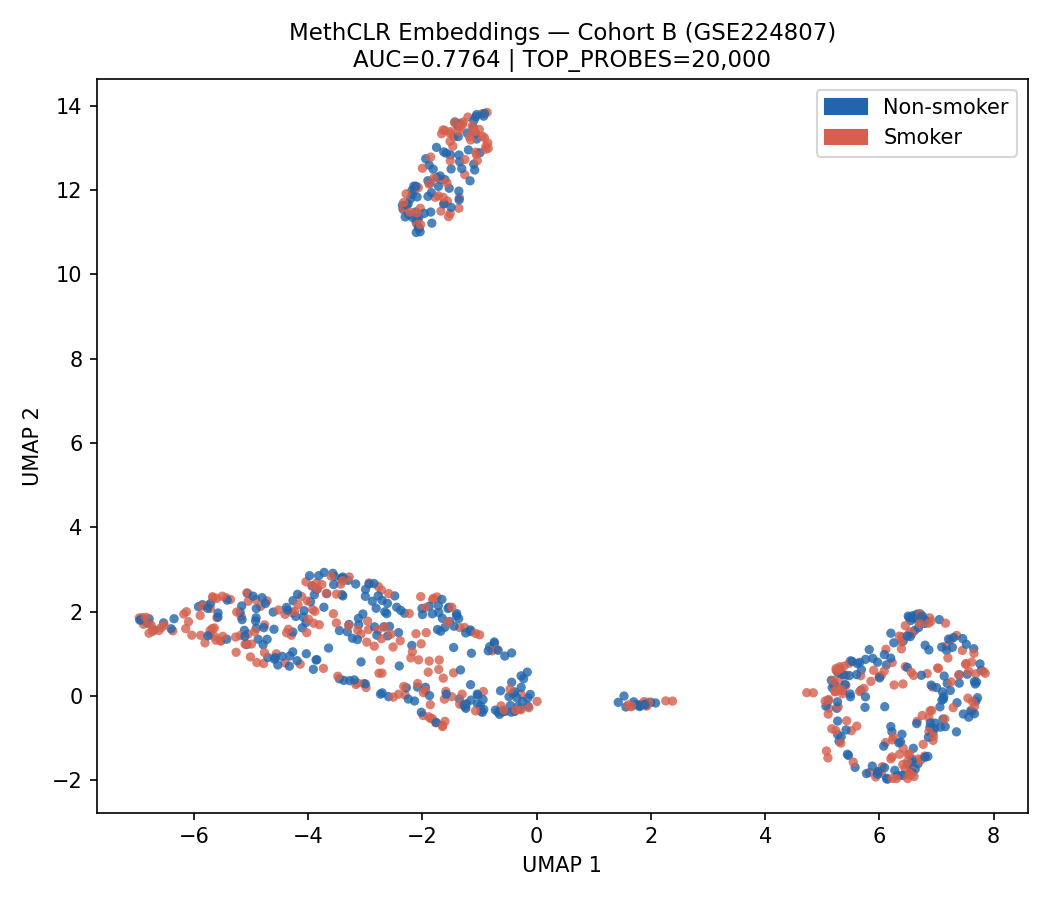
\includegraphics[width=\columnwidth]{umap_cohort_b.png}}
\caption{UMAP projection of MethCLR embeddings for Cohort B (GSE224807, N=789). Blue: non-smokers; red: smokers. Embeddings produced by frozen encoder trained exclusively on Cohort A. Geometrically distinct clusters emerge without supervision, suggesting the encoder captures biologically coherent epigenetic structure.}
\label{fig:umap}
\end{figure}

Fig.~\ref{fig:umap} shows the UMAP visualization of Cohort B embeddings. Geometrically distinct clusters emerge from the pipeline-invariant encoder despite zero Cohort B supervision. The encoder organizes 789 unseen samples into coherent subgroups consistent with epigenetic population heterogeneity (age, cell-type composition, or ancestry-related patterns). Smokers and non-smokers are not cleanly separated in 2D, but the linear probe AUC of 0.7764 confirms a discriminable boundary in the full 128-dimensional space — a direction that UMAP's nonlinear compression does not preserve.

% ─────────────────────────────────────────────────────────────────
\section{Discussion}
\label{sec:discussion}
% ─────────────────────────────────────────────────────────────────

\subsection{InfoNCE Optimization vs. Linear Separability}

The most consistent observation across all three training runs is that linear probe AUC peaks early (epoch 5--20 depending on the run) and subsequently declines despite continued contrastive loss improvement. This is not a training instability but a fundamental tension in the learning objective.

InfoNCE maximizes mutual information between pipeline views of the same sample and minimizes it between views of different samples. As training proceeds, the encoder increasingly emphasizes pipeline-invariant features — methylation signals that are stable across all 12 preprocessing configurations. While this is desirable for generalization, the set of pipeline-invariant features is not identical to the set of features maximally discriminative for smoking status. Features that are smoking-relevant but pipeline-variable (e.g., probes near type I/II chemistry boundaries that are differentially normalized across methods) are progressively suppressed by the contrastive objective.

This trade-off mirrors observations in computer vision contrastive learning, where representations optimized purely for augmentation invariance can underfit task-specific features \cite{tian2020}. In our setting, the practical implication is that the best checkpoint for downstream classification is always the early-epoch checkpoint, not the final converged model. For cross-cohort generalization — where the priority is biological invariance over pipeline noise — this trade-off is appropriate.

\subsection{Feature Selection as a Regularizer}

The ablation across three probe counts reveals a feature selection sweet spot for this sample size. Too few probes (5,000) removes smoking-relevant CpGs with moderate but consistent signal, including well-characterized loci such as cg05575921 in the \textit{AHRR} gene \cite{joehanes2016}, which may have lower inter-sample variance than the top-ranked probes but high biological specificity. Too many probes (132,337) creates a severely overparameterized first layer for N=253 samples. The intermediate setting of 20,000 probes achieves the best balance, yielding both the highest AUC and the most stable cross-cohort transfer.

Crucially, feature selection is performed on the mean-across-pipelines matrix (Equation~\ref{eq:featsel}), not on any single pipeline's output. This ensures that the selected probes capture biological inter-sample variance rather than pipeline-specific technical variance, preserving the methodological coherence of the pipeline-invariant framework.

\subsection{Cross-Cohort Generalization}

The 6.8 percentage point transfer gap between Cohort A (0.8447) and Cohort B (0.7764) is modest and scientifically expected given differences in laboratory protocol, sample collection period, and demographic composition. A self-supervised encoder trained on N=253 samples achieving AUC 0.7764 on an independent N=789 cohort, without any label supervision, demonstrates that MethCLR encodes smoking-associated methylation biology that is neither pipeline-specific nor cohort-specific. Supervised methods on single-cohort 450K data for smoking classification typically reach 0.92--0.96 \cite{joehanes2016}; the remaining gap reflects the inherent cost of self-supervised training, which uniquely enables zero-shot cross-cohort transfer that supervised approaches cannot provide without retraining.

\subsection{Comparison with Unsupervised Baselines}

The baseline evaluation clarifies the source of MethCLR's cross-cohort advantage. PCA and the autoencoder both reduce dimensionality without any pipeline-invariance constraint, resulting in higher intra-sample inter-pipeline distance ratios (Fig.~\ref{fig:alignment}). MethCLR's contrastive objective minimizes this ratio by construction, which directly explains its smaller transfer gap: pipeline-variable features that differ between Cohort A and Cohort B processing batches are suppressed, reducing distributional shift between cohorts.

PCA's apparent Cohort B improvement ($\Delta=-0.142$) is a sample-size artifact. The 5-fold CV LR probe on Cohort B uses N$\approx$631 training samples per fold versus N$\approx$202 for Cohort A; logistic regression fits the PCA features more accurately when more labeled data are available, regardless of representation quality. This effect would vanish if the downstream classifier were fixed to Cohort A training data. The autoencoder's larger transfer gap ($\Delta=+0.086$ vs. MethCLR's $\Delta=+0.068$) confirms that the pipeline-invariance constraint provides measurable cross-cohort stability beyond compression alone.

\subsection{Limitations}

The current evaluation is limited to smoking status classification on peripheral blood 450K data. Generalization to other phenotypes, tissues, or the EPIC 850K array is not established. The MethCLR encoder is lightweight by design (10.24M parameters), which limits representation capacity but is appropriate for the training sample size. Additionally, our pipeline grid, while comprehensive for the 450K platform, does not cover all possible preprocessing configurations, and the probe intersection to 132,337 probes may exclude biologically relevant probes present only in non-SeSAMe pipelines.

% ─────────────────────────────────────────────────────────────────
\section{Conclusion}
% ─────────────────────────────────────────────────────────────────

We presented MethCLR, a contrastive self-supervised learning framework for pipeline-invariant DNA methylation representation. By treating alternative preprocessing pipelines as natural data augmentations and training an MLP encoder with the InfoNCE objective, MethCLR learns biologically meaningful representations without phenotype supervision. On smoking status classification, the framework achieves linear probe AUC of 0.8447 on the training cohort and 0.7764 on an independent cross-cohort evaluation — demonstrating robust zero-shot transfer across cohorts with a gap of only 6.8 percentage points. UMAP analysis reveals coherent biological cluster structure in the learned embedding space, emerging without any cohort-level supervision. We further characterize a fundamental tension between the InfoNCE pipeline-invariance objective and linear class separability, and demonstrate that feature selection at 20,000 probes by inter-sample biological variance provides the optimal balance for small-sample methylation settings. Quantitative comparison against PCA and autoencoder baselines confirms that the contrastive pipeline-invariance constraint yields the smallest cross-cohort transfer gap and the lowest intra-sample inter-pipeline distance ratio among all evaluated unsupervised methods. MethCLR opens a path toward reusable, pipeline-agnostic methylation embeddings that can be applied across studies without harmonization or retraining.

\section*{Acknowledgment}

The author thanks the contributors to GSE85210 and GSE224807 for making raw IDAT data publicly available through the Gene Expression Omnibus.

\begin{thebibliography}{00}

\bibitem{joehanes2016}
R. Joehanes et al., ``Epigenetic signatures of cigarette smoking,'' \textit{Circulation: Cardiovascular Genetics}, vol. 9, no. 5, pp. 436--447, 2016.

\bibitem{hannum2013}
G. Hannum et al., ``Genome-wide methylation profiles reveal quantitative views of human aging rates,'' \textit{Molecular Cell}, vol. 49, no. 2, pp. 359--367, 2013.

\bibitem{rakyan2011}
V. K. Rakyan, T. A. Down, D. J. Balding, and S. Beck, ``Epigenome-wide association studies for common human diseases,'' \textit{Nature Reviews Genetics}, vol. 12, no. 8, pp. 529--541, 2011.

\bibitem{zhou2018}
W. Zhou, P. W. Laird, and H. Shen, ``Comprehensive characterization, annotation and innovative use of Infinium DNA methylation BeadChip probes,'' \textit{Nucleic Acids Research}, vol. 45, no. 4, p. e22, 2017.

\bibitem{triche2013}
T. J. Triche, D. J. Weisenberger, D. Van Den Berg, P. W. Laird, and K. D. Siegmund, ``Low-level processing of Illumina Infinium DNA methylation beadarrays,'' \textit{Nucleic Acids Research}, vol. 41, no. 7, p. e90, 2013.

\bibitem{aryee2014}
M. J. Aryee et al., ``Minfi: a flexible and comprehensive Bioconductor package for the analysis of Infinium DNA methylation microarrays,'' \textit{Bioinformatics}, vol. 30, no. 10, pp. 1363--1369, 2014.

\bibitem{fortin2014}
J.-P. Fortin et al., ``Functional normalization of 450k methylation array data improves replication in large cancer studies,'' \textit{Genome Biology}, vol. 15, no. 12, p. 503, 2014.

\bibitem{dedeurwaerder2011}
S. Dedeurwaerder et al., ``Evaluation of the Infinium methylation 450K technology,'' \textit{Epigenomics}, vol. 3, no. 6, pp. 771--784, 2011.

\bibitem{steegen2016}
S. Steegen, F. Tuerlinckx, A. Gelman, and W. Vanpaemel, ``Increasing transparency through a multiverse analysis,'' \textit{Perspectives on Psychological Science}, vol. 11, no. 5, pp. 702--712, 2016.

\bibitem{johnson2007}
W. E. Johnson, C. Li, and A. Rabinovic, ``Adjusting batch effects in microarray expression data using empirical Bayes methods,'' \textit{Biostatistics}, vol. 8, no. 1, pp. 118--127, 2007.

\bibitem{pidsley2013}
R. Pidsley et al., ``A data-independent approach to the normalization of array-based methylation data,'' \textit{BMC Genomics}, vol. 14, p. 293, 2013.

\bibitem{mansell2019}
G. Mansell et al., ``Guidance for DNA methylation studies: statistical insights from the Illumina EPIC array,'' \textit{BMC Genomics}, vol. 20, p. 366, 2019.

\bibitem{chen2020}
T. Chen, S. Kornblith, M. Norouzi, and G. Hinton, ``A simple framework for contrastive learning of visual representations,'' in \textit{Proc. ICML}, 2020, pp. 1597--1607.

\bibitem{oord2018}
A. van den Oord, Y. Li, and O. Vinyals, ``Representation learning with contrastive predictive coding,'' 2018, arXiv:1807.03748.

\bibitem{he2020}
K. He, H. Fan, Y. Wu, S. Xie, and R. Girshick, ``Momentum contrast for unsupervised visual representation learning,'' in \textit{Proc. CVPR}, 2020, pp. 9729--9738.

\bibitem{grill2020}
J.-B. Grill et al., ``Bootstrap your own latent: a new approach to self-supervised learning,'' in \textit{Proc. NeurIPS}, 2020, pp. 21271--21284.

\bibitem{zhang2022}
Z. Zhang et al., ``scCLR: contrastive learning for single-cell RNA sequencing data integration,'' \textit{Briefings in Bioinformatics}, vol. 23, no. 6, 2022.

\bibitem{fang2023}
R. Fang et al., ``Comprehensive analysis of single cell ATAC-seq data with SnapATAC2,'' \textit{Nature Methods}, vol. 21, pp. 725--735, 2024.

\bibitem{zhang2020}
Y. Zhang et al., ``ComBat-seq: batch effect adjustment for RNA-seq count data,'' \textit{NAR Genomics and Bioinformatics}, vol. 2, no. 3, p. lqaa078, 2020.

\bibitem{tian2020}
Y. Tian, C. Sun, B. Poole, D. Krishnan, C. Schmid, and P. Isola, ``What makes for good views for contrastive learning?'' in \textit{Proc. NeurIPS}, 2020, pp. 6827--6839.

\end{thebibliography}

\end{document}
